\documentclass[1p]{elsarticle_modified}
%\bibliographystyle{elsarticle-num}

%\usepackage[colorlinks]{hyperref}
%\usepackage{abbrmath_seonhwa} %\Abb, \Ascr, \Acal ,\Abf, \Afrak
\usepackage{amsfonts}
\usepackage{amssymb}
\usepackage{amsmath}
\usepackage{amsthm}
\usepackage{scalefnt}
\usepackage{amsbsy}
\usepackage{kotex}
\usepackage{caption}
\usepackage{subfig}
\usepackage{color}
\usepackage{graphicx}
\usepackage{xcolor} %% white, black, red, green, blue, cyan, magenta, yellow
\usepackage{float}
\usepackage{setspace}
\usepackage{hyperref}

\usepackage{tikz}
\usetikzlibrary{arrows}

\usepackage{multirow}
\usepackage{array} % fixed length table
\usepackage{hhline}

%%%%%%%%%%%%%%%%%%%%%
\makeatletter
\renewcommand*\env@matrix[1][\arraystretch]{%
	\edef\arraystretch{#1}%
	\hskip -\arraycolsep
	\let\@ifnextchar\new@ifnextchar
	\array{*\c@MaxMatrixCols c}}
\makeatother %https://tex.stackexchange.com/questions/14071/how-can-i-increase-the-line-spacing-in-a-matrix
%%%%%%%%%%%%%%%

\usepackage[normalem]{ulem}

\newcommand{\msout}[1]{\ifmmode\text{\sout{\ensuremath{#1}}}\else\sout{#1}\fi}
%SOURCE: \msout is \stkout macro in https://tex.stackexchange.com/questions/20609/strikeout-in-math-mode

\newcommand{\cancel}[1]{
	\ifmmode
	{\color{red}\msout{#1}}
	\else
	{\color{red}\sout{#1}}
	\fi
}

\newcommand{\add}[1]{
	{\color{blue}\uwave{#1}}
}

\newcommand{\replace}[2]{
	\ifmmode
	{\color{red}\msout{#1}}{\color{blue}\uwave{#2}}
	\else
	{\color{red}\sout{#1}}{\color{blue}\uwave{#2}}
	\fi
}

\newcommand{\Sol}{\mathcal{S}} %segment
\newcommand{\D}{D} %diagram
\newcommand{\A}{\mathcal{A}} %arc


%%%%%%%%%%%%%%%%%%%%%%%%%%%%%5 test

\def\sl{\operatorname{\textup{SL}}(2,\Cbb)}
\def\psl{\operatorname{\textup{PSL}}(2,\Cbb)}
\def\quan{\mkern 1mu \triangleright \mkern 1mu}

\theoremstyle{definition}
\newtheorem{thm}{Theorem}[section]
\newtheorem{prop}[thm]{Proposition}
\newtheorem{lem}[thm]{Lemma}
\newtheorem{ques}[thm]{Question}
\newtheorem{cor}[thm]{Corollary}
\newtheorem{defn}[thm]{Definition}
\newtheorem{exam}[thm]{Example}
\newtheorem{rmk}[thm]{Remark}
\newtheorem{alg}[thm]{Algorithm}

\newcommand{\I}{\sqrt{-1}}
\begin{document}

%\begin{frontmatter}
%
%\title{Boundary parabolic representations of knots up to 8 crossings}
%
%%% Group authors per affiliation:
%\author{Yunhi Cho} 
%\address{Department of Mathematics, University of Seoul, Seoul, Korea}
%\ead{yhcho@uos.ac.kr}
%
%
%\author{Seonhwa Kim} %\fnref{s_kim}}
%\address{Center for Geometry and Physics, Institute for Basic Science, Pohang, 37673, Korea}
%\ead{ryeona17@ibs.re.kr}
%
%\author{Hyuk Kim}
%\address{Department of Mathematical Sciences, Seoul National University, Seoul 08826, Korea}
%\ead{hyukkim@snu.ac.kr}
%
%\author{Seokbeom Yoon}
%\address{Department of Mathematical Sciences, Seoul National University, Seoul, 08826,  Korea}
%\ead{sbyoon15@snu.ac.kr}
%
%\begin{abstract}
%We find all boundary parabolic representation of knots up to 8 crossings.
%
%\end{abstract}
%\begin{keyword}
%    \MSC[2010] 57M25 
%\end{keyword}
%
%\end{frontmatter}

%\linenumbers
%\tableofcontents
%
\newcommand\colored[1]{\textcolor{white}{\rule[-0.35ex]{0.8em}{1.4ex}}\kern-0.8em\color{red} #1}%
%\newcommand\colored[1]{\textcolor{white}{ #1}\kern-2.17ex	\textcolor{white}{ #1}\kern-1.81ex	\textcolor{white}{ #1}\kern-2.15ex\color{red}#1	}

{\Large $\underline{12a_{0179}~(K12a_{0179})}$}

\setlength{\tabcolsep}{10pt}
\renewcommand{\arraystretch}{1.6}
\vspace{1cm}\begin{tabular}{m{100pt}>{\centering\arraybackslash}m{274pt}}
\multirow{5}{120pt}{
	\centering
	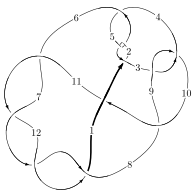
\includegraphics[width=112pt]{../../../GIT/diagram.site/Diagrams/png/980_12a_0179.png}\\
\ \ \ A knot diagram\footnotemark}&
\allowdisplaybreaks
\textbf{Linearized knot diagam} \\
\cline{2-2}
 &
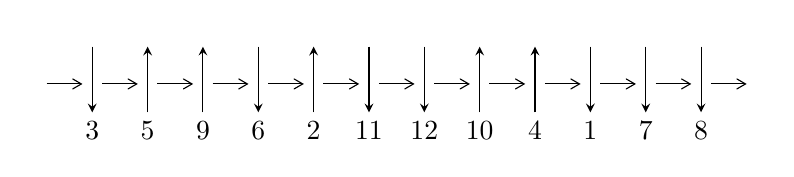
\begin{tikzpicture}[x=20pt, y=17pt]
	% nodes
	\node (C0) at (0, 0) {};
	\node (C1) at (1, 0) {};
	\node (C1U) at (1, +1) {};
	\node (C1D) at (1, -1) {3};

	\node (C2) at (2, 0) {};
	\node (C2U) at (2, +1) {};
	\node (C2D) at (2, -1) {5};

	\node (C3) at (3, 0) {};
	\node (C3U) at (3, +1) {};
	\node (C3D) at (3, -1) {9};

	\node (C4) at (4, 0) {};
	\node (C4U) at (4, +1) {};
	\node (C4D) at (4, -1) {6};

	\node (C5) at (5, 0) {};
	\node (C5U) at (5, +1) {};
	\node (C5D) at (5, -1) {2};

	\node (C6) at (6, 0) {};
	\node (C6U) at (6, +1) {};
	\node (C6D) at (6, -1) {11};

	\node (C7) at (7, 0) {};
	\node (C7U) at (7, +1) {};
	\node (C7D) at (7, -1) {12};

	\node (C8) at (8, 0) {};
	\node (C8U) at (8, +1) {};
	\node (C8D) at (8, -1) {10};

	\node (C9) at (9, 0) {};
	\node (C9U) at (9, +1) {};
	\node (C9D) at (9, -1) {4};

	\node (C10) at (10, 0) {};
	\node (C10U) at (10, +1) {};
	\node (C10D) at (10, -1) {1};

	\node (C11) at (11, 0) {};
	\node (C11U) at (11, +1) {};
	\node (C11D) at (11, -1) {7};

	\node (C12) at (12, 0) {};
	\node (C12U) at (12, +1) {};
	\node (C12D) at (12, -1) {8};
	\node (C13) at (13, 0) {};

	% arrows
	\draw[->,>={angle 60}]
	(C0) edge (C1) (C1) edge (C2) (C2) edge (C3) (C3) edge (C4) (C4) edge (C5) (C5) edge (C6) (C6) edge (C7) (C7) edge (C8) (C8) edge (C9) (C9) edge (C10) (C10) edge (C11) (C11) edge (C12) (C12) edge (C13) ;	\draw[->,>=stealth]
	(C1U) edge (C1D) (C2D) edge (C2U) (C3D) edge (C3U) (C4U) edge (C4D) (C5D) edge (C5U) (C6U) edge (C6D) (C7U) edge (C7D) (C8D) edge (C8U) (C9D) edge (C9U) (C10U) edge (C10D) (C11U) edge (C11D) (C12U) edge (C12D) ;
	\end{tikzpicture} \\
\hhline{~~} \\& 
\textbf{Solving Sequence} \\ \cline{2-2} 
 &
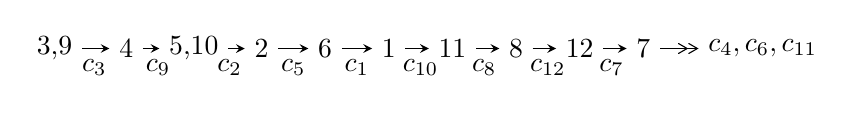
\begin{tikzpicture}[x=23pt, y=7pt]
	% node
	\node (A0) at (-1/8, 0) {3,9};
	\node (A1) at (1, 0) {4};
	\node (A2) at (33/16, 0) {5,10};
	\node (A3) at (25/8, 0) {2};
	\node (A4) at (33/8, 0) {6};
	\node (A5) at (41/8, 0) {1};
	\node (A6) at (49/8, 0) {11};
	\node (A7) at (57/8, 0) {8};
	\node (A8) at (65/8, 0) {12};
	\node (A9) at (73/8, 0) {7};
	\node (C1) at (1/2, -1) {$c_{3}$};
	\node (C2) at (3/2, -1) {$c_{9}$};
	\node (C3) at (21/8, -1) {$c_{2}$};
	\node (C4) at (29/8, -1) {$c_{5}$};
	\node (C5) at (37/8, -1) {$c_{1}$};
	\node (C6) at (45/8, -1) {$c_{10}$};
	\node (C7) at (53/8, -1) {$c_{8}$};
	\node (C8) at (61/8, -1) {$c_{12}$};
	\node (C9) at (69/8, -1) {$c_{7}$};
	\node (A10) at (11, 0) {$c_{4},c_{6},c_{11}$};

	% edge
	\draw[->,>=stealth]	
	(A0) edge (A1) (A1) edge (A2) (A2) edge (A3) (A3) edge (A4) (A4) edge (A5) (A5) edge (A6) (A6) edge (A7) (A7) edge (A8) (A8) edge (A9) ;
	\draw[->>,>={angle 60}]	
	(A9) edge (A10);
\end{tikzpicture} \\ 

\end{tabular} \\

\footnotetext{
The image of knot diagram is generated by the software ``\textbf{Draw programme}" developed by Andrew Bartholomew(\url{http://www.layer8.co.uk/maths/draw/index.htm\#Running-draw}), where we modified some parts for our purpose(\url{https://github.com/CATsTAILs/LinksPainter}).
}\phantom \\ \newline 
\centering \textbf{Ideals for irreducible components\footnotemark of $X_{\text{par}}$} 
 
\begin{align*}
I^u_{1}&=\langle 
-2.71708\times10^{39} u^{70}+1.91637\times10^{39} u^{69}+\cdots+7.55053\times10^{39} b-5.39067\times10^{40},\\
\phantom{I^u_{1}}&\phantom{= \langle  }2.23600\times10^{39} u^{70}+3.25449\times10^{37} u^{69}+\cdots+7.55053\times10^{39} a+2.20656\times10^{40},\;u^{71}- u^{70}+\cdots+32 u-16\rangle \\
\\
I^v_{1}&=\langle 
a,\;- v^3+2 v^2+2 b-2 v+1,\;v^4- v^3+2 v^2+v+1\rangle \\
\end{align*}
\raggedright * 2 irreducible components of $\dim_{\mathbb{C}}=0$, with total 75 representations.\\
\footnotetext{All coefficients of polynomials are rational numbers. But the coefficients are sometimes approximated in decimal forms when there is not enough margin.}
\newpage
\renewcommand{\arraystretch}{1}
\centering \section*{I. $I^u_{1}= \langle -2.72\times10^{39} u^{70}+1.92\times10^{39} u^{69}+\cdots+7.55\times10^{39} b-5.39\times10^{40},\;2.24\times10^{39} u^{70}+3.25\times10^{37} u^{69}+\cdots+7.55\times10^{39} a+2.21\times10^{40},\;u^{71}- u^{70}+\cdots+32 u-16 \rangle$}
\flushleft \textbf{(i) Arc colorings}\\
\begin{tabular}{m{7pt} m{180pt} m{7pt} m{180pt} }
\flushright $a_{3}=$&$\begin{pmatrix}1\\0\end{pmatrix}$ \\
\flushright $a_{9}=$&$\begin{pmatrix}0\\u\end{pmatrix}$ \\
\flushright $a_{4}=$&$\begin{pmatrix}1\\- u^2\end{pmatrix}$ \\
\flushright $a_{5}=$&$\begin{pmatrix}-0.296138 u^{70}-0.00431028 u^{69}+\cdots+12.0993 u-2.92239\\0.359852 u^{70}-0.253806 u^{69}+\cdots-4.10423 u+7.13946\end{pmatrix}$ \\
\flushright $a_{10}=$&$\begin{pmatrix}u\\- u^3+u\end{pmatrix}$ \\
\flushright $a_{2}=$&$\begin{pmatrix}-0.0672794 u^{70}-0.0679694 u^{69}+\cdots+9.94426 u-3.79346\\-0.204932 u^{70}-0.00949976 u^{69}+\cdots-0.840329 u-3.24825\end{pmatrix}$ \\
\flushright $a_{6}=$&$\begin{pmatrix}-0.0672794 u^{70}-0.0679694 u^{69}+\cdots+9.94426 u-3.79346\\0.114199 u^{70}-0.134587 u^{69}+\cdots-2.41116 u+5.41223\end{pmatrix}$ \\
\flushright $a_{1}=$&$\begin{pmatrix}-0.272212 u^{70}-0.0774692 u^{69}+\cdots+9.10394 u-7.04171\\-0.204932 u^{70}-0.00949976 u^{69}+\cdots-0.840329 u-3.24825\end{pmatrix}$ \\
\flushright $a_{11}=$&$\begin{pmatrix}0.0361174 u^{70}-0.0228612 u^{69}+\cdots+12.0016 u-6.74339\\-0.0426249 u^{70}-0.173546 u^{69}+\cdots-2.35671 u+4.17575\end{pmatrix}$ \\
\flushright $a_{8}=$&$\begin{pmatrix}- u^3\\u^5- u^3+u\end{pmatrix}$ \\
\flushright $a_{12}=$&$\begin{pmatrix}-0.169607 u^{70}+0.0192873 u^{69}+\cdots+9.80052 u-8.54872\\-0.197794 u^{70}+0.101478 u^{69}+\cdots-2.00512 u-2.63268\end{pmatrix}$ \\
\flushright $a_{7}=$&$\begin{pmatrix}0.184380 u^{70}-0.0878898 u^{69}+\cdots-13.0143 u+10.6308\\0.288200 u^{70}-0.111556 u^{69}+\cdots+0.409843 u+3.14069\end{pmatrix}$\\&\end{tabular}
\flushleft \textbf{(ii) Obstruction class $= -1$}\\~\\
\flushleft \textbf{(iii) Cusp Shapes $= 1.56249 u^{70}-0.499654 u^{69}+\cdots-24.3357 u+56.8547$}\\~\\
\newpage\renewcommand{\arraystretch}{1}
\flushleft \textbf{(iv) u-Polynomials at the component}\newline \\
\begin{tabular}{m{50pt}|m{274pt}}
Crossings & \hspace{64pt}u-Polynomials at each crossing \\
\hline $$\begin{aligned}c_{1},c_{4}\end{aligned}$$&$\begin{aligned}
&u^{71}+25 u^{70}+\cdots-24 u-1
\end{aligned}$\\
\hline $$\begin{aligned}c_{2},c_{5}\end{aligned}$$&$\begin{aligned}
&u^{71}+3 u^{70}+\cdots-12 u^2-1
\end{aligned}$\\
\hline $$\begin{aligned}c_{3},c_{9}\end{aligned}$$&$\begin{aligned}
&u^{71}+u^{70}+\cdots+32 u+16
\end{aligned}$\\
\hline $$\begin{aligned}c_{6},c_{7},c_{11}\\c_{12}\end{aligned}$$&$\begin{aligned}
&u^{71}+3 u^{70}+\cdots-2 u+1
\end{aligned}$\\
\hline $$\begin{aligned}c_{8}\end{aligned}$$&$\begin{aligned}
&u^{71}-25 u^{70}+\cdots+3712 u-256
\end{aligned}$\\
\hline $$\begin{aligned}c_{10}\end{aligned}$$&$\begin{aligned}
&u^{71}-21 u^{70}+\cdots+30122 u-2513
\end{aligned}$\\
\hline
\end{tabular}\\~\\
\newpage\renewcommand{\arraystretch}{1}
\flushleft \textbf{(v) Riley Polynomials at the component}\newline \\
\begin{tabular}{m{50pt}|m{274pt}}
Crossings & \hspace{64pt}Riley Polynomials at each crossing \\
\hline $$\begin{aligned}c_{1},c_{4}\end{aligned}$$&$\begin{aligned}
&y^{71}+45 y^{70}+\cdots+32 y-1
\end{aligned}$\\
\hline $$\begin{aligned}c_{2},c_{5}\end{aligned}$$&$\begin{aligned}
&y^{71}+25 y^{70}+\cdots-24 y-1
\end{aligned}$\\
\hline $$\begin{aligned}c_{3},c_{9}\end{aligned}$$&$\begin{aligned}
&y^{71}-25 y^{70}+\cdots+3712 y-256
\end{aligned}$\\
\hline $$\begin{aligned}c_{6},c_{7},c_{11}\\c_{12}\end{aligned}$$&$\begin{aligned}
&y^{71}-83 y^{70}+\cdots+4 y-1
\end{aligned}$\\
\hline $$\begin{aligned}c_{8}\end{aligned}$$&$\begin{aligned}
&y^{71}+35 y^{70}+\cdots-1695744 y-65536
\end{aligned}$\\
\hline $$\begin{aligned}c_{10}\end{aligned}$$&$\begin{aligned}
&y^{71}-23 y^{70}+\cdots+38952656 y-6315169
\end{aligned}$\\
\hline
\end{tabular}\\~\\
\newpage\flushleft \textbf{(vi) Complex Volumes and Cusp Shapes}
$$\begin{array}{c|c|c}  
\text{Solutions to }I^u_{1}& \I (\text{vol} + \sqrt{-1}CS) & \text{Cusp shape}\\
 \hline 
\begin{aligned}
u &= \phantom{-}0.898695 + 0.447888 I \\
a &= -0.48166 + 1.64393 I \\
b &= \phantom{-}0.704202 - 0.678389 I\end{aligned}
 & -0.156625 - 0.128245 I & -2.60256 + 0.62828 I \\ \hline\begin{aligned}
u &= \phantom{-}0.898695 - 0.447888 I \\
a &= -0.48166 - 1.64393 I \\
b &= \phantom{-}0.704202 + 0.678389 I\end{aligned}
 & -0.156625 + 0.128245 I & -2.60256 - 0.62828 I \\ \hline\begin{aligned}
u &= \phantom{-}0.485356 + 0.866096 I \\
a &= \phantom{-}0.723279 - 0.275133 I \\
b &= -0.695289 - 0.658546 I\end{aligned}
 & -0.181303 - 0.963321 I & -2.97724 + 2.47393 I \\ \hline\begin{aligned}
u &= \phantom{-}0.485356 - 0.866096 I \\
a &= \phantom{-}0.723279 + 0.275133 I \\
b &= -0.695289 + 0.658546 I\end{aligned}
 & -0.181303 + 0.963321 I & -2.97724 - 2.47393 I \\ \hline\begin{aligned}
u &= -0.046756 + 1.006700 I \\
a &= \phantom{-}0.664918 - 0.351532 I \\
b &= -0.707383 - 0.856092 I\end{aligned}
 & -4.78280 + 2.70516 I & -3.93532 - 3.08025 I \\ \hline\begin{aligned}
u &= -0.046756 - 1.006700 I \\
a &= \phantom{-}0.664918 + 0.351532 I \\
b &= -0.707383 + 0.856092 I\end{aligned}
 & -4.78280 - 2.70516 I & -3.93532 + 3.08025 I \\ \hline\begin{aligned}
u &= \phantom{-}0.814841 + 0.602433 I \\
a &= -2.85625 + 1.03972 I \\
b &= \phantom{-}0.633904 + 0.996625 I\end{aligned}
 & -9.92867 + 3.79379 I & -6.79831 - 6.12485 I \\ \hline\begin{aligned}
u &= \phantom{-}0.814841 - 0.602433 I \\
a &= -2.85625 - 1.03972 I \\
b &= \phantom{-}0.633904 - 0.996625 I\end{aligned}
 & -9.92867 - 3.79379 I & -6.79831 + 6.12485 I \\ \hline\begin{aligned}
u &= \phantom{-}1.03416\phantom{ +0.000000I} \\
a &= \phantom{-}0.792535\phantom{ +0.000000I} \\
b &= -0.659001\phantom{ +0.000000I}\end{aligned}
 & -4.08496\phantom{ +0.000000I} & \phantom{-0.000000 } 0 \\ \hline\begin{aligned}
u &= \phantom{-}0.915846 + 0.508550 I \\
a &= \phantom{-}0.777578 - 0.138252 I \\
b &= -0.671992 - 0.337720 I\end{aligned}
 & \phantom{-}0.04777 + 3.88882 I & \phantom{-0.000000 } 0. - 7.52926 I\\
 \hline 
 \end{array}$$\newpage$$\begin{array}{c|c|c}  
\text{Solutions to }I^u_{1}& \I (\text{vol} + \sqrt{-1}CS) & \text{Cusp shape}\\
 \hline 
\begin{aligned}
u &= \phantom{-}0.915846 - 0.508550 I \\
a &= \phantom{-}0.777578 + 0.138252 I \\
b &= -0.671992 + 0.337720 I\end{aligned}
 & \phantom{-}0.04777 - 3.88882 I & \phantom{-0.000000 -}0. + 7.52926 I \\ \hline\begin{aligned}
u &= -0.749394 + 0.742501 I \\
a &= \phantom{-}0.927602 + 1.023970 I \\
b &= -0.002922 + 1.034700 I\end{aligned}
 & -5.23643 + 0.49136 I & -10.35637 + 0. I\phantom{ +0.000000I} \\ \hline\begin{aligned}
u &= -0.749394 - 0.742501 I \\
a &= \phantom{-}0.927602 - 1.023970 I \\
b &= -0.002922 - 1.034700 I\end{aligned}
 & -5.23643 - 0.49136 I & -10.35637 + 0. I\phantom{ +0.000000I} \\ \hline\begin{aligned}
u &= \phantom{-}0.842164 + 0.647596 I \\
a &= \phantom{-}0.860044 - 0.892957 I \\
b &= -0.080620 - 1.043370 I\end{aligned}
 & -2.69671 + 2.52237 I & \phantom{-0.000000 } 0 \\ \hline\begin{aligned}
u &= \phantom{-}0.842164 - 0.647596 I \\
a &= \phantom{-}0.860044 + 0.892957 I \\
b &= -0.080620 + 1.043370 I\end{aligned}
 & -2.69671 - 2.52237 I & \phantom{-0.000000 } 0 \\ \hline\begin{aligned}
u &= -0.744352 + 0.553739 I \\
a &= \phantom{-}0.651043 - 0.469715 I \\
b &= -0.561912 - 1.022170 I\end{aligned}
 & -1.79172 + 0.68850 I & -5.62900 + 3.38039 I \\ \hline\begin{aligned}
u &= -0.744352 - 0.553739 I \\
a &= \phantom{-}0.651043 + 0.469715 I \\
b &= -0.561912 + 1.022170 I\end{aligned}
 & -1.79172 - 0.68850 I & -5.62900 - 3.38039 I \\ \hline\begin{aligned}
u &= -0.913780 + 0.144906 I \\
a &= \phantom{-}0.731500 + 0.609419 I \\
b &= -0.338962 + 1.033540 I\end{aligned}
 & -7.19330 - 3.32362 I & -5.12286 + 4.83275 I \\ \hline\begin{aligned}
u &= -0.913780 - 0.144906 I \\
a &= \phantom{-}0.731500 - 0.609419 I \\
b &= -0.338962 - 1.033540 I\end{aligned}
 & -7.19330 + 3.32362 I & -5.12286 - 4.83275 I \\ \hline\begin{aligned}
u &= \phantom{-}0.895328 + 0.614559 I \\
a &= \phantom{-}0.627473 + 0.478230 I \\
b &= -0.571721 + 1.063660 I\end{aligned}
 & -9.66637 + 1.00404 I & \phantom{-0.000000 } 0\\
 \hline 
 \end{array}$$\newpage$$\begin{array}{c|c|c}  
\text{Solutions to }I^u_{1}& \I (\text{vol} + \sqrt{-1}CS) & \text{Cusp shape}\\
 \hline 
\begin{aligned}
u &= \phantom{-}0.895328 - 0.614559 I \\
a &= \phantom{-}0.627473 - 0.478230 I \\
b &= -0.571721 - 1.063660 I\end{aligned}
 & -9.66637 - 1.00404 I & \phantom{-0.000000 } 0 \\ \hline\begin{aligned}
u &= -0.580986 + 0.928128 I \\
a &= \phantom{-}0.629379 - 0.415842 I \\
b &= -0.663444 - 0.995696 I\end{aligned}
 & -1.18425 + 6.22847 I & \phantom{-0.000000 } 0 \\ \hline\begin{aligned}
u &= -0.580986 - 0.928128 I \\
a &= \phantom{-}0.629379 + 0.415842 I \\
b &= -0.663444 + 0.995696 I\end{aligned}
 & -1.18425 - 6.22847 I & \phantom{-0.000000 } 0 \\ \hline\begin{aligned}
u &= \phantom{-}0.438808 + 0.779885 I \\
a &= \phantom{-}0.657294 + 0.414809 I \\
b &= -0.631199 + 0.953782 I\end{aligned}
 & \phantom{-}0.39399 - 3.06003 I & -0.75932 + 1.65602 I \\ \hline\begin{aligned}
u &= \phantom{-}0.438808 - 0.779885 I \\
a &= \phantom{-}0.657294 - 0.414809 I \\
b &= -0.631199 - 0.953782 I\end{aligned}
 & \phantom{-}0.39399 + 3.06003 I & -0.75932 - 1.65602 I \\ \hline\begin{aligned}
u &= \phantom{-}0.731479 + 0.831783 I \\
a &= \phantom{-}0.88446 - 1.13386 I \\
b &= \phantom{-}0.038927 - 1.065800 I\end{aligned}
 & -13.52330 - 2.24339 I & \phantom{-0.000000 } 0 \\ \hline\begin{aligned}
u &= \phantom{-}0.731479 - 0.831783 I \\
a &= \phantom{-}0.88446 + 1.13386 I \\
b &= \phantom{-}0.038927 + 1.065800 I\end{aligned}
 & -13.52330 + 2.24339 I & \phantom{-0.000000 } 0 \\ \hline\begin{aligned}
u &= -0.955053 + 0.565034 I \\
a &= -2.56607 - 0.59068 I \\
b &= \phantom{-}0.670926 - 0.992762 I\end{aligned}
 & -1.10321 - 5.18739 I & \phantom{-0.000000 } 0 \\ \hline\begin{aligned}
u &= -0.955053 - 0.565034 I \\
a &= -2.56607 + 0.59068 I \\
b &= \phantom{-}0.670926 + 0.992762 I\end{aligned}
 & -1.10321 + 5.18739 I & \phantom{-0.000000 } 0 \\ \hline\begin{aligned}
u &= -0.821890 + 0.297804 I \\
a &= \phantom{-}0.838078 + 0.097095 I \\
b &= -0.543921 + 0.231319 I\end{aligned}
 & \phantom{-}1.32332 - 0.80569 I & \phantom{-}4.20345 + 1.04258 I\\
 \hline 
 \end{array}$$\newpage$$\begin{array}{c|c|c}  
\text{Solutions to }I^u_{1}& \I (\text{vol} + \sqrt{-1}CS) & \text{Cusp shape}\\
 \hline 
\begin{aligned}
u &= -0.821890 - 0.297804 I \\
a &= \phantom{-}0.838078 - 0.097095 I \\
b &= -0.543921 - 0.231319 I\end{aligned}
 & \phantom{-}1.32332 + 0.80569 I & \phantom{-}4.20345 - 1.04258 I \\ \hline\begin{aligned}
u &= -0.595799 + 0.966991 I \\
a &= \phantom{-}0.704626 + 0.251056 I \\
b &= -0.754441 + 0.629987 I\end{aligned}
 & -7.86275 + 2.84728 I & \phantom{-0.000000 } 0 \\ \hline\begin{aligned}
u &= -0.595799 - 0.966991 I \\
a &= \phantom{-}0.704626 - 0.251056 I \\
b &= -0.754441 - 0.629987 I\end{aligned}
 & -7.86275 - 2.84728 I & \phantom{-0.000000 } 0 \\ \hline\begin{aligned}
u &= -0.943340 + 0.686884 I \\
a &= \phantom{-}0.769346 + 0.904490 I \\
b &= -0.091008 + 1.099760 I\end{aligned}
 & -4.63880 - 5.93106 I & \phantom{-0.000000 } 0 \\ \hline\begin{aligned}
u &= -0.943340 - 0.686884 I \\
a &= \phantom{-}0.769346 - 0.904490 I \\
b &= -0.091008 - 1.099760 I\end{aligned}
 & -4.63880 + 5.93106 I & \phantom{-0.000000 } 0 \\ \hline\begin{aligned}
u &= -0.995858 + 0.614315 I \\
a &= \phantom{-}0.744700 + 0.143172 I \\
b &= -0.745958 + 0.363151 I\end{aligned}
 & -7.64756 - 5.89043 I & \phantom{-0.000000 } 0 \\ \hline\begin{aligned}
u &= -0.995858 - 0.614315 I \\
a &= \phantom{-}0.744700 - 0.143172 I \\
b &= -0.745958 - 0.363151 I\end{aligned}
 & -7.64756 + 5.89043 I & \phantom{-0.000000 } 0 \\ \hline\begin{aligned}
u &= -1.185220 + 0.024512 I \\
a &= -1.68390 - 0.91780 I \\
b &= \phantom{-}0.763748 + 0.846463 I\end{aligned}
 & \phantom{-}6.09381 + 0.94811 I & \phantom{-0.000000 } 0 \\ \hline\begin{aligned}
u &= -1.185220 - 0.024512 I \\
a &= -1.68390 + 0.91780 I \\
b &= \phantom{-}0.763748 - 0.846463 I\end{aligned}
 & \phantom{-}6.09381 - 0.94811 I & \phantom{-0.000000 } 0 \\ \hline\begin{aligned}
u &= \phantom{-}1.190440 + 0.117078 I \\
a &= -1.91536 - 0.66291 I \\
b &= \phantom{-}0.755383 + 0.886674 I\end{aligned}
 & \phantom{-}5.97207 + 4.78145 I & \phantom{-0.000000 } 0\\
 \hline 
 \end{array}$$\newpage$$\begin{array}{c|c|c}  
\text{Solutions to }I^u_{1}& \I (\text{vol} + \sqrt{-1}CS) & \text{Cusp shape}\\
 \hline 
\begin{aligned}
u &= \phantom{-}1.190440 - 0.117078 I \\
a &= -1.91536 + 0.66291 I \\
b &= \phantom{-}0.755383 - 0.886674 I\end{aligned}
 & \phantom{-}5.97207 - 4.78145 I & \phantom{-0.000000 } 0 \\ \hline\begin{aligned}
u &= \phantom{-}0.660911 + 1.000500 I \\
a &= \phantom{-}0.615402 + 0.416919 I \\
b &= -0.678388 + 1.018840 I\end{aligned}
 & -9.01807 - 8.30674 I & \phantom{-0.000000 } 0 \\ \hline\begin{aligned}
u &= \phantom{-}0.660911 - 1.000500 I \\
a &= \phantom{-}0.615402 - 0.416919 I \\
b &= -0.678388 - 1.018840 I\end{aligned}
 & -9.01807 + 8.30674 I & \phantom{-0.000000 } 0 \\ \hline\begin{aligned}
u &= -0.639037 + 0.480316 I \\
a &= \phantom{-}0.63082 - 2.00324 I \\
b &= \phantom{-}0.578600 + 0.637489 I\end{aligned}
 & -8.84566 + 1.15303 I & -4.74959 + 2.27232 I \\ \hline\begin{aligned}
u &= -0.639037 - 0.480316 I \\
a &= \phantom{-}0.63082 + 2.00324 I \\
b &= \phantom{-}0.578600 - 0.637489 I\end{aligned}
 & -8.84566 - 1.15303 I & -4.74959 - 2.27232 I \\ \hline\begin{aligned}
u &= -1.066010 + 0.557376 I \\
a &= -0.553984 - 1.154100 I \\
b &= \phantom{-}0.783980 + 0.661621 I\end{aligned}
 & \phantom{-}3.27242 - 2.74628 I & \phantom{-0.000000 } 0 \\ \hline\begin{aligned}
u &= -1.066010 - 0.557376 I \\
a &= -0.553984 + 1.154100 I \\
b &= \phantom{-}0.783980 - 0.661621 I\end{aligned}
 & \phantom{-}3.27242 + 2.74628 I & \phantom{-0.000000 } 0 \\ \hline\begin{aligned}
u &= -0.216560 + 0.759366 I \\
a &= \phantom{-}0.723009 + 0.336172 I \\
b &= -0.635057 + 0.763179 I\end{aligned}
 & \phantom{-}1.00588 - 1.89636 I & \phantom{-}0.54641 + 5.25437 I \\ \hline\begin{aligned}
u &= -0.216560 - 0.759366 I \\
a &= \phantom{-}0.723009 - 0.336172 I \\
b &= -0.635057 - 0.763179 I\end{aligned}
 & \phantom{-}1.00588 + 1.89636 I & \phantom{-}0.54641 - 5.25437 I \\ \hline\begin{aligned}
u &= \phantom{-}1.217720 + 0.204604 I \\
a &= -1.28956 + 1.01899 I \\
b &= \phantom{-}0.788740 - 0.796172 I\end{aligned}
 & -0.028361 + 1.390240 I & \phantom{-0.000000 } 0\\
 \hline 
 \end{array}$$\newpage$$\begin{array}{c|c|c}  
\text{Solutions to }I^u_{1}& \I (\text{vol} + \sqrt{-1}CS) & \text{Cusp shape}\\
 \hline 
\begin{aligned}
u &= \phantom{-}1.217720 - 0.204604 I \\
a &= -1.28956 - 1.01899 I \\
b &= \phantom{-}0.788740 + 0.796172 I\end{aligned}
 & -0.028361 - 1.390240 I & \phantom{-0.000000 } 0 \\ \hline\begin{aligned}
u &= \phantom{-}0.998362 + 0.733734 I \\
a &= \phantom{-}0.720523 - 0.920806 I \\
b &= -0.086327 - 1.133430 I\end{aligned}
 & -12.6856 + 8.1034 I & \phantom{-0.000000 } 0 \\ \hline\begin{aligned}
u &= \phantom{-}0.998362 - 0.733734 I \\
a &= \phantom{-}0.720523 + 0.920806 I \\
b &= -0.086327 + 1.133430 I\end{aligned}
 & -12.6856 - 8.1034 I & \phantom{-0.000000 } 0 \\ \hline\begin{aligned}
u &= \phantom{-}1.075840 + 0.632701 I \\
a &= -2.18572 + 0.55812 I \\
b &= \phantom{-}0.698464 + 1.015000 I\end{aligned}
 & \phantom{-}2.20770 + 8.35369 I & \phantom{-0.000000 } 0 \\ \hline\begin{aligned}
u &= \phantom{-}1.075840 - 0.632701 I \\
a &= -2.18572 - 0.55812 I \\
b &= \phantom{-}0.698464 - 1.015000 I\end{aligned}
 & \phantom{-}2.20770 - 8.35369 I & \phantom{-0.000000 } 0 \\ \hline\begin{aligned}
u &= -1.223810 + 0.275921 I \\
a &= -1.99796 + 0.29578 I \\
b &= \phantom{-}0.754446 - 0.931385 I\end{aligned}
 & -0.43731 - 7.18811 I & \phantom{-0.000000 } 0 \\ \hline\begin{aligned}
u &= -1.223810 - 0.275921 I \\
a &= -1.99796 - 0.29578 I \\
b &= \phantom{-}0.754446 + 0.931385 I\end{aligned}
 & -0.43731 + 7.18811 I & \phantom{-0.000000 } 0 \\ \hline\begin{aligned}
u &= -0.422944 + 0.589272 I \\
a &= \phantom{-}1.234610 - 0.617787 I \\
b &= \phantom{-}0.389148 + 0.464716 I\end{aligned}
 & -8.91534 + 1.12808 I & -7.69562 + 1.51946 I \\ \hline\begin{aligned}
u &= -0.422944 - 0.589272 I \\
a &= \phantom{-}1.234610 + 0.617787 I \\
b &= \phantom{-}0.389148 - 0.464716 I\end{aligned}
 & -8.91534 - 1.12808 I & -7.69562 - 1.51946 I \\ \hline\begin{aligned}
u &= \phantom{-}1.093130 + 0.656674 I \\
a &= -0.464088 + 1.005390 I \\
b &= \phantom{-}0.811468 - 0.632359 I\end{aligned}
 & \phantom{-}1.65039 + 6.56883 I & \phantom{-0.000000 } 0\\
 \hline 
 \end{array}$$\newpage$$\begin{array}{c|c|c}  
\text{Solutions to }I^u_{1}& \I (\text{vol} + \sqrt{-1}CS) & \text{Cusp shape}\\
 \hline 
\begin{aligned}
u &= \phantom{-}1.093130 - 0.656674 I \\
a &= -0.464088 - 1.005390 I \\
b &= \phantom{-}0.811468 + 0.632359 I\end{aligned}
 & \phantom{-}1.65039 - 6.56883 I & \phantom{-0.000000 } 0 \\ \hline\begin{aligned}
u &= -1.098940 + 0.711938 I \\
a &= -2.03891 - 0.66504 I \\
b &= \phantom{-}0.700760 - 1.035720 I\end{aligned}
 & \phantom{-}0.43518 - 12.25320 I & \phantom{-0.000000 } 0 \\ \hline\begin{aligned}
u &= -1.098940 - 0.711938 I \\
a &= -2.03891 + 0.66504 I \\
b &= \phantom{-}0.700760 + 1.035720 I\end{aligned}
 & \phantom{-}0.43518 + 12.25320 I & \phantom{-0.000000 } 0 \\ \hline\begin{aligned}
u &= -1.106240 + 0.731732 I \\
a &= -0.410040 - 0.912009 I \\
b &= \phantom{-}0.831200 + 0.610202 I\end{aligned}
 & -6.25111 - 9.04376 I & \phantom{-0.000000 } 0 \\ \hline\begin{aligned}
u &= -1.106240 - 0.731732 I \\
a &= -0.410040 + 0.912009 I \\
b &= \phantom{-}0.831200 - 0.610202 I\end{aligned}
 & -6.25111 + 9.04376 I & \phantom{-0.000000 } 0 \\ \hline\begin{aligned}
u &= \phantom{-}1.106610 + 0.773513 I \\
a &= -1.94318 + 0.74250 I \\
b &= \phantom{-}0.700048 + 1.051230 I\end{aligned}
 & -7.5826 + 14.7744 I & \phantom{-0.000000 } 0 \\ \hline\begin{aligned}
u &= \phantom{-}1.106610 - 0.773513 I \\
a &= -1.94318 - 0.74250 I \\
b &= \phantom{-}0.700048 - 1.051230 I\end{aligned}
 & -7.5826 - 14.7744 I & \phantom{-0.000000 } 0 \\ \hline\begin{aligned}
u &= \phantom{-}0.595380 + 0.063159 I \\
a &= \phantom{-}0.766930 - 0.508281 I \\
b &= -0.410411 - 0.925666 I\end{aligned}
 & -0.52089 + 2.54938 I & \phantom{-}1.55851 - 8.99527 I \\ \hline\begin{aligned}
u &= \phantom{-}0.595380 - 0.063159 I \\
a &= \phantom{-}0.766930 + 0.508281 I \\
b &= -0.410411 + 0.925666 I\end{aligned}
 & -0.52089 - 2.54938 I & \phantom{-}1.55851 + 8.99527 I \\ \hline\begin{aligned}
u &= \phantom{-}0.327964 + 0.426910 I \\
a &= \phantom{-}1.107820 + 0.038370 I \\
b &= \phantom{-}0.096513 - 0.298186 I\end{aligned}
 & -1.159260 - 0.383261 I & -7.97768 + 0.90492 I\\
 \hline 
 \end{array}$$\newpage$$\begin{array}{c|c|c}  
\text{Solutions to }I^u_{1}& \I (\text{vol} + \sqrt{-1}CS) & \text{Cusp shape}\\
 \hline 
\begin{aligned}
u &= \phantom{-}0.327964 - 0.426910 I \\
a &= \phantom{-}1.107820 - 0.038370 I \\
b &= \phantom{-}0.096513 + 0.298186 I\end{aligned}
 & -1.159260 + 0.383261 I & -7.97768 - 0.90492 I\\
 \hline 
 \end{array}$$\newpage\newpage\renewcommand{\arraystretch}{1}
\centering \section*{II. $I^v_{1}= \langle a,\;- v^3+2 v^2+2 b-2 v+1,\;v^4- v^3+2 v^2+v+1 \rangle$}
\flushleft \textbf{(i) Arc colorings}\\
\begin{tabular}{m{7pt} m{180pt} m{7pt} m{180pt} }
\flushright $a_{3}=$&$\begin{pmatrix}1\\0\end{pmatrix}$ \\
\flushright $a_{9}=$&$\begin{pmatrix}v\\0\end{pmatrix}$ \\
\flushright $a_{4}=$&$\begin{pmatrix}1\\0\end{pmatrix}$ \\
\flushright $a_{5}=$&$\begin{pmatrix}0\\\frac{1}{2} v^3- v^2+v-\frac{1}{2}\end{pmatrix}$ \\
\flushright $a_{10}=$&$\begin{pmatrix}v\\0\end{pmatrix}$ \\
\flushright $a_{2}=$&$\begin{pmatrix}1\\-\frac{1}{2} v^3+v^2- v-\frac{1}{2}\end{pmatrix}$ \\
\flushright $a_{6}=$&$\begin{pmatrix}\frac{1}{2} v^3- v^2+v-\frac{1}{2}\\\frac{1}{2} v^3- v^2+v+\frac{1}{2}\end{pmatrix}$ \\
\flushright $a_{1}=$&$\begin{pmatrix}-\frac{1}{2} v^3+v^2- v+\frac{1}{2}\\-\frac{1}{2} v^3+v^2- v-\frac{1}{2}\end{pmatrix}$ \\
\flushright $a_{11}=$&$\begin{pmatrix}0\\-\frac{1}{2} v^3- v-\frac{1}{2}\end{pmatrix}$ \\
\flushright $a_{8}=$&$\begin{pmatrix}v\\0\end{pmatrix}$ \\
\flushright $a_{12}=$&$\begin{pmatrix}- v\\-\frac{1}{2} v^3+v^2- v-\frac{1}{2}\end{pmatrix}$ \\
\flushright $a_{7}=$&$\begin{pmatrix}\frac{1}{2} v^3- v^2+v-\frac{1}{2}\\\frac{1}{2} v^3+v+\frac{1}{2}\end{pmatrix}$\\&\end{tabular}
\flushleft \textbf{(ii) Obstruction class $= 1$}\\~\\
\flushleft \textbf{(iii) Cusp Shapes $= v^3-3 v^2+v-7$}\\~\\
\newpage\renewcommand{\arraystretch}{1}
\flushleft \textbf{(iv) u-Polynomials at the component}\newline \\
\begin{tabular}{m{50pt}|m{274pt}}
Crossings & \hspace{64pt}u-Polynomials at each crossing \\
\hline $$\begin{aligned}c_{1},c_{4},c_{5}\end{aligned}$$&$\begin{aligned}
&(u^2- u+1)^2
\end{aligned}$\\
\hline $$\begin{aligned}c_{2}\end{aligned}$$&$\begin{aligned}
&(u^2+u+1)^2
\end{aligned}$\\
\hline $$\begin{aligned}c_{3},c_{8},c_{9}\end{aligned}$$&$\begin{aligned}
&u^4
\end{aligned}$\\
\hline $$\begin{aligned}c_{6},c_{7},c_{10}\end{aligned}$$&$\begin{aligned}
&(u^2+u-1)^2
\end{aligned}$\\
\hline $$\begin{aligned}c_{11},c_{12}\end{aligned}$$&$\begin{aligned}
&(u^2- u-1)^2
\end{aligned}$\\
\hline
\end{tabular}\\~\\
\newpage\renewcommand{\arraystretch}{1}
\flushleft \textbf{(v) Riley Polynomials at the component}\newline \\
\begin{tabular}{m{50pt}|m{274pt}}
Crossings & \hspace{64pt}Riley Polynomials at each crossing \\
\hline $$\begin{aligned}c_{1},c_{2},c_{4}\\c_{5}\end{aligned}$$&$\begin{aligned}
&(y^2+y+1)^2
\end{aligned}$\\
\hline $$\begin{aligned}c_{3},c_{8},c_{9}\end{aligned}$$&$\begin{aligned}
&y^4
\end{aligned}$\\
\hline $$\begin{aligned}c_{6},c_{7},c_{10}\\c_{11},c_{12}\end{aligned}$$&$\begin{aligned}
&(y^2-3 y+1)^2
\end{aligned}$\\
\hline
\end{tabular}\\~\\
\newpage\flushleft \textbf{(vi) Complex Volumes and Cusp Shapes}
$$\begin{array}{c|c|c}  
\text{Solutions to }I^v_{1}& \I (\text{vol} + \sqrt{-1}CS) & \text{Cusp shape}\\
 \hline 
\begin{aligned}
v &= -0.309017 + 0.535233 I \\
a &= \phantom{-0.000000 } 0 \\
b &= -0.500000 + 0.866025 I\end{aligned}
 & -0.98696 - 2.02988 I & -6.50000 + 1.52761 I \\ \hline\begin{aligned}
v &= -0.309017 - 0.535233 I \\
a &= \phantom{-0.000000 } 0 \\
b &= -0.500000 - 0.866025 I\end{aligned}
 & -0.98696 + 2.02988 I & -6.50000 - 1.52761 I \\ \hline\begin{aligned}
v &= \phantom{-}0.80902 + 1.40126 I \\
a &= \phantom{-0.000000 } 0 \\
b &= -0.500000 - 0.866025 I\end{aligned}
 & -8.88264 + 2.02988 I & -6.50000 - 5.40059 I \\ \hline\begin{aligned}
v &= \phantom{-}0.80902 - 1.40126 I \\
a &= \phantom{-0.000000 } 0 \\
b &= -0.500000 + 0.866025 I\end{aligned}
 & -8.88264 - 2.02988 I & -6.50000 + 5.40059 I\\
 \hline 
 \end{array}$$\newpage
\newpage\renewcommand{\arraystretch}{1}
\centering \section*{ III. u-Polynomials}
\begin{tabular}{m{50pt}|m{274pt}}
Crossings & \hspace{64pt}u-Polynomials at each crossing \\
\hline $$\begin{aligned}c_{1},c_{4}\end{aligned}$$&$\begin{aligned}
&((u^2- u+1)^2)(u^{71}+25 u^{70}+\cdots-24 u-1)
\end{aligned}$\\
\hline $$\begin{aligned}c_{2}\end{aligned}$$&$\begin{aligned}
&((u^2+u+1)^2)(u^{71}+3 u^{70}+\cdots-12 u^2-1)
\end{aligned}$\\
\hline $$\begin{aligned}c_{3},c_{9}\end{aligned}$$&$\begin{aligned}
&u^4(u^{71}+u^{70}+\cdots+32 u+16)
\end{aligned}$\\
\hline $$\begin{aligned}c_{5}\end{aligned}$$&$\begin{aligned}
&((u^2- u+1)^2)(u^{71}+3 u^{70}+\cdots-12 u^2-1)
\end{aligned}$\\
\hline $$\begin{aligned}c_{6},c_{7}\end{aligned}$$&$\begin{aligned}
&((u^2+u-1)^2)(u^{71}+3 u^{70}+\cdots-2 u+1)
\end{aligned}$\\
\hline $$\begin{aligned}c_{8}\end{aligned}$$&$\begin{aligned}
&u^4(u^{71}-25 u^{70}+\cdots+3712 u-256)
\end{aligned}$\\
\hline $$\begin{aligned}c_{10}\end{aligned}$$&$\begin{aligned}
&((u^2+u-1)^2)(u^{71}-21 u^{70}+\cdots+30122 u-2513)
\end{aligned}$\\
\hline $$\begin{aligned}c_{11},c_{12}\end{aligned}$$&$\begin{aligned}
&((u^2- u-1)^2)(u^{71}+3 u^{70}+\cdots-2 u+1)
\end{aligned}$\\
\hline
\end{tabular}\newpage\renewcommand{\arraystretch}{1}
\centering \section*{ IV. Riley Polynomials}
\begin{tabular}{m{50pt}|m{274pt}}
Crossings & \hspace{64pt}Riley Polynomials at each crossing \\
\hline $$\begin{aligned}c_{1},c_{4}\end{aligned}$$&$\begin{aligned}
&((y^2+y+1)^2)(y^{71}+45 y^{70}+\cdots+32 y-1)
\end{aligned}$\\
\hline $$\begin{aligned}c_{2},c_{5}\end{aligned}$$&$\begin{aligned}
&((y^2+y+1)^2)(y^{71}+25 y^{70}+\cdots-24 y-1)
\end{aligned}$\\
\hline $$\begin{aligned}c_{3},c_{9}\end{aligned}$$&$\begin{aligned}
&y^4(y^{71}-25 y^{70}+\cdots+3712 y-256)
\end{aligned}$\\
\hline $$\begin{aligned}c_{6},c_{7},c_{11}\\c_{12}\end{aligned}$$&$\begin{aligned}
&((y^2-3 y+1)^2)(y^{71}-83 y^{70}+\cdots+4 y-1)
\end{aligned}$\\
\hline $$\begin{aligned}c_{8}\end{aligned}$$&$\begin{aligned}
&y^4(y^{71}+35 y^{70}+\cdots-1695744 y-65536)
\end{aligned}$\\
\hline $$\begin{aligned}c_{10}\end{aligned}$$&$\begin{aligned}
&((y^2-3 y+1)^2)(y^{71}-23 y^{70}+\cdots+3.89527\times10^{7} y-6315169)
\end{aligned}$\\
\hline
\end{tabular}
\vskip 2pc
\end{document}